\chapter{Wireframe}
\label{cha:Wireframe}

Um \textit{wireframe} é um protótipo da interface do sistema, que serve para ilustrar o funcionamento e interação do usuário com o sistema. A seguir estão três telas do sistema: a página inicial, a página de criação de grade horária, e a página de avaliação de disciplinas e professores. Essas são as principais páginas do sistema.

\begin{figure}[ht]
    \begin{center}
    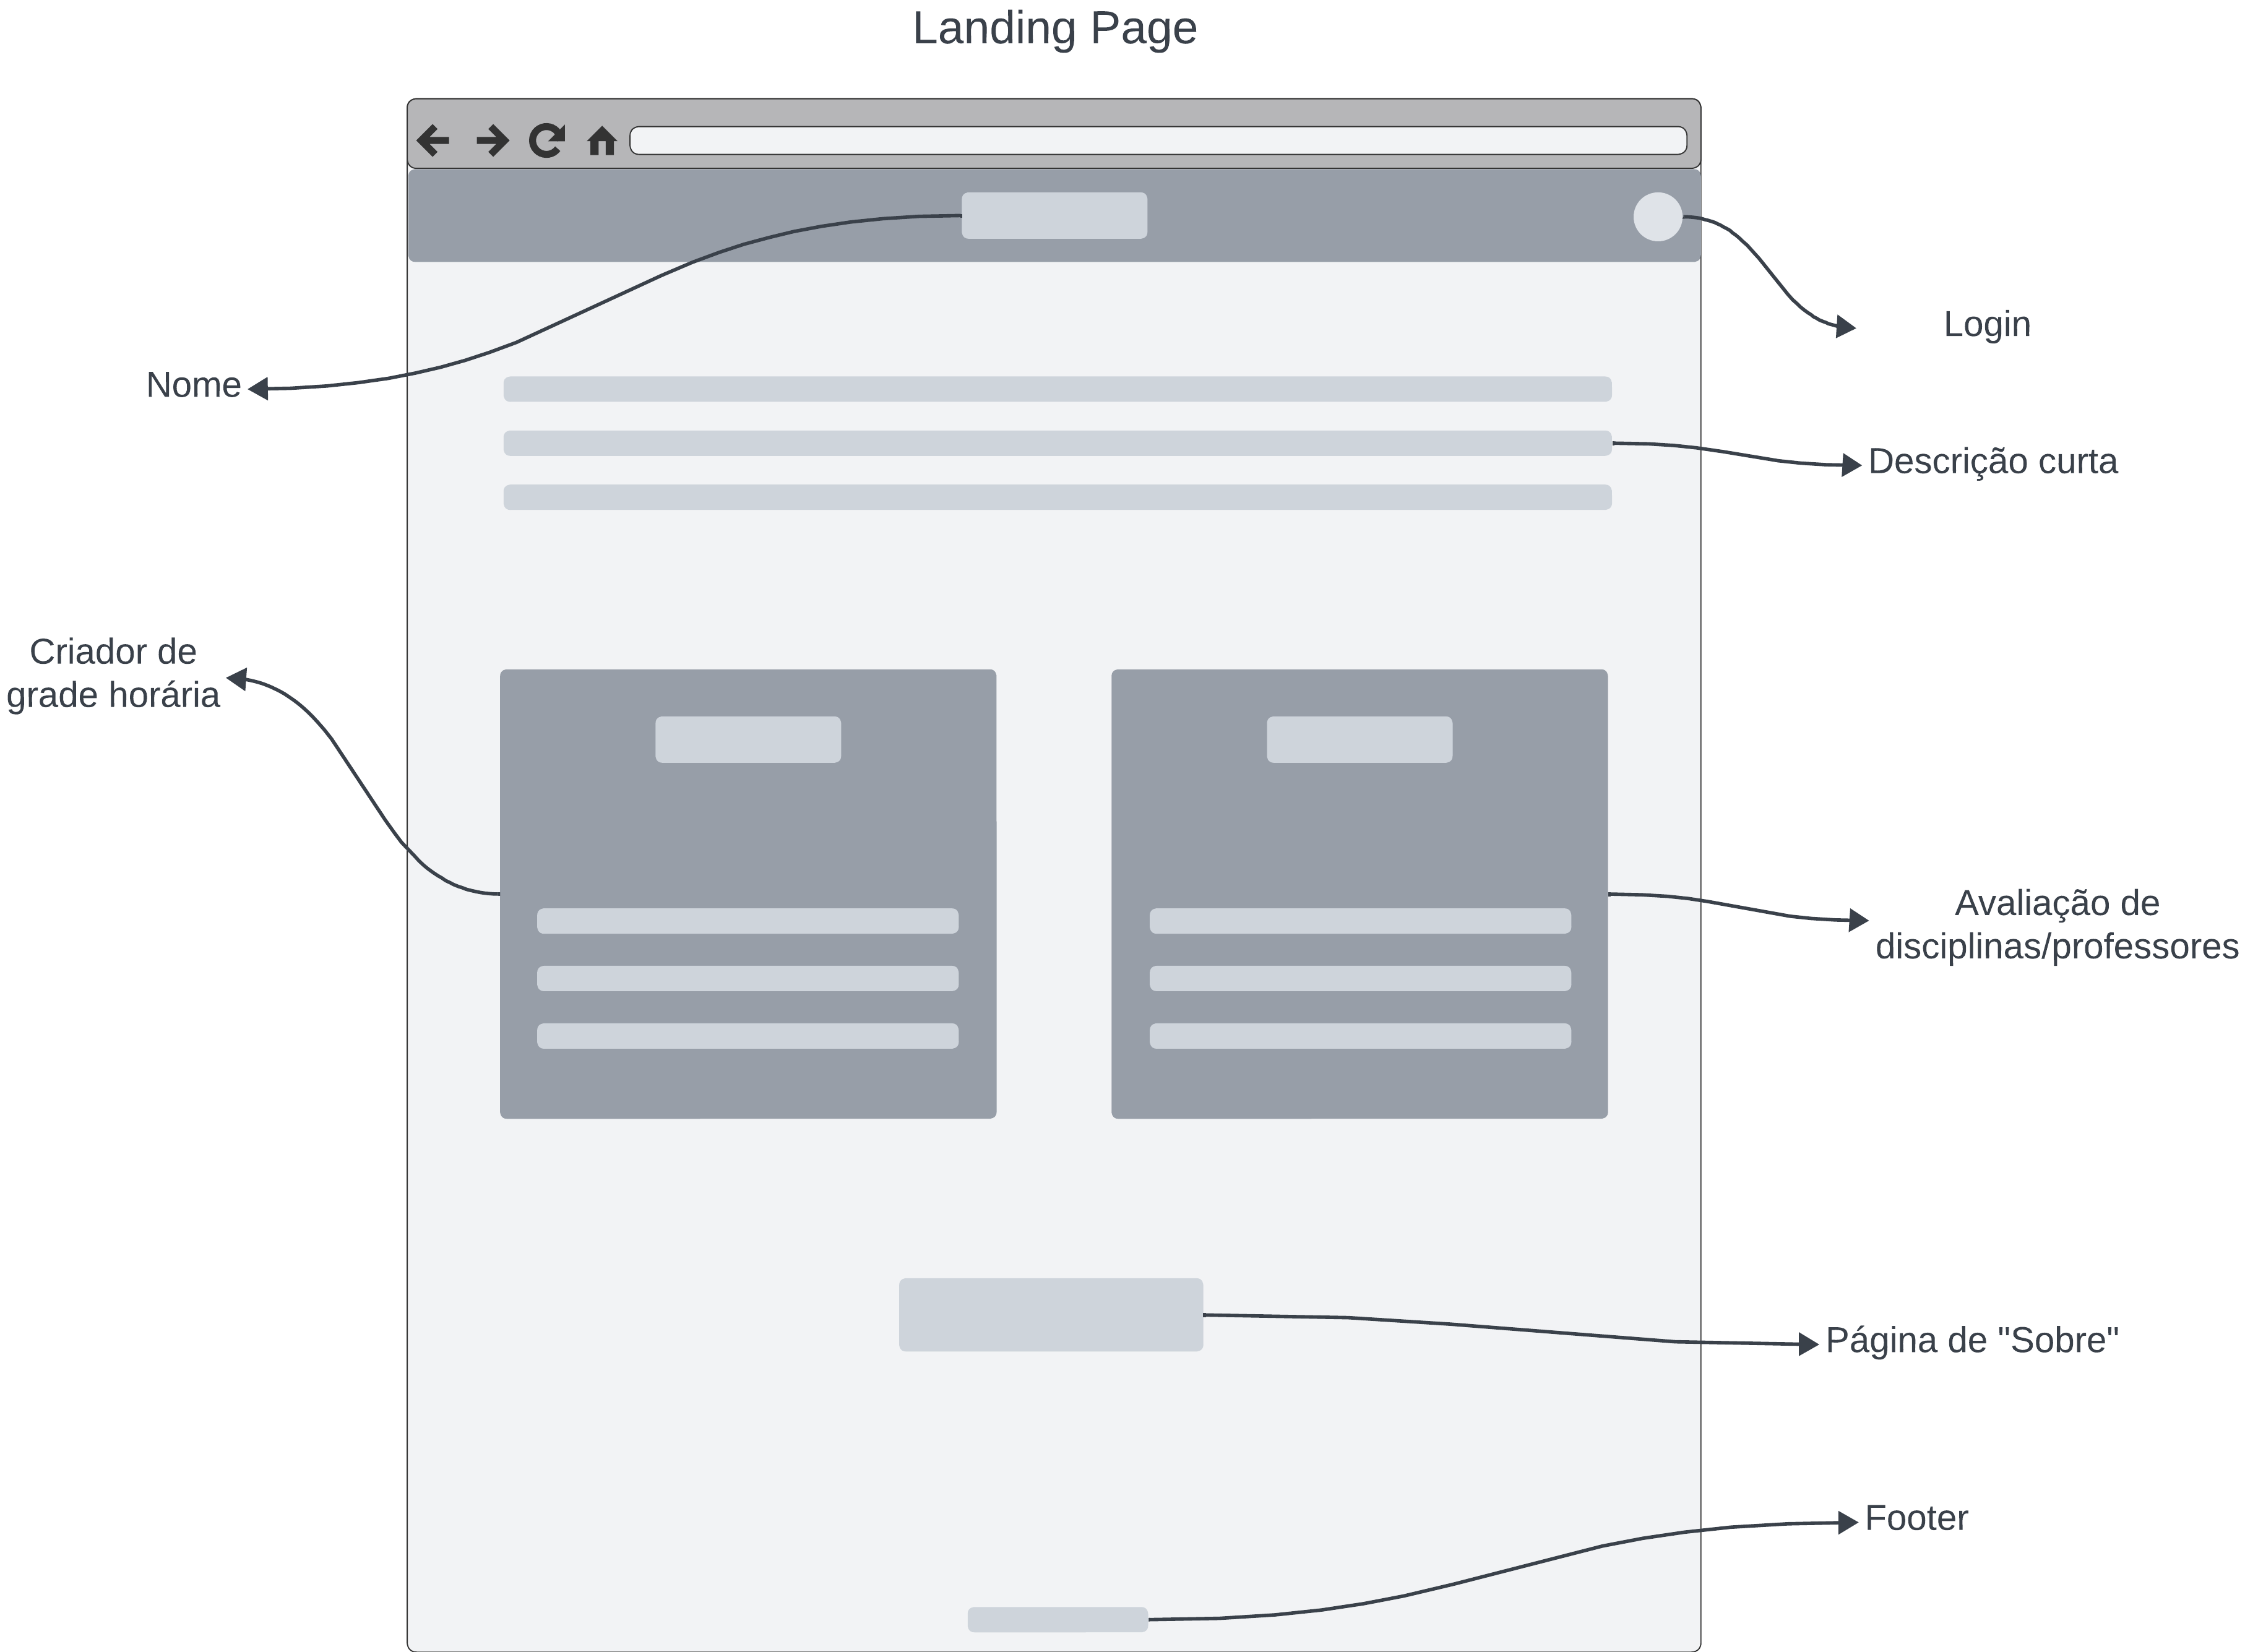
\includegraphics[width=390pt]{figuras/pagina-inicial.png}
    \caption{Wireframe da página inicial (\textit{Landing Page})}
    \label{fig:wireframe-pagina-inicial}
    \end{center}
\end{figure}

\begin{figure}[ht]
    \begin{center}
    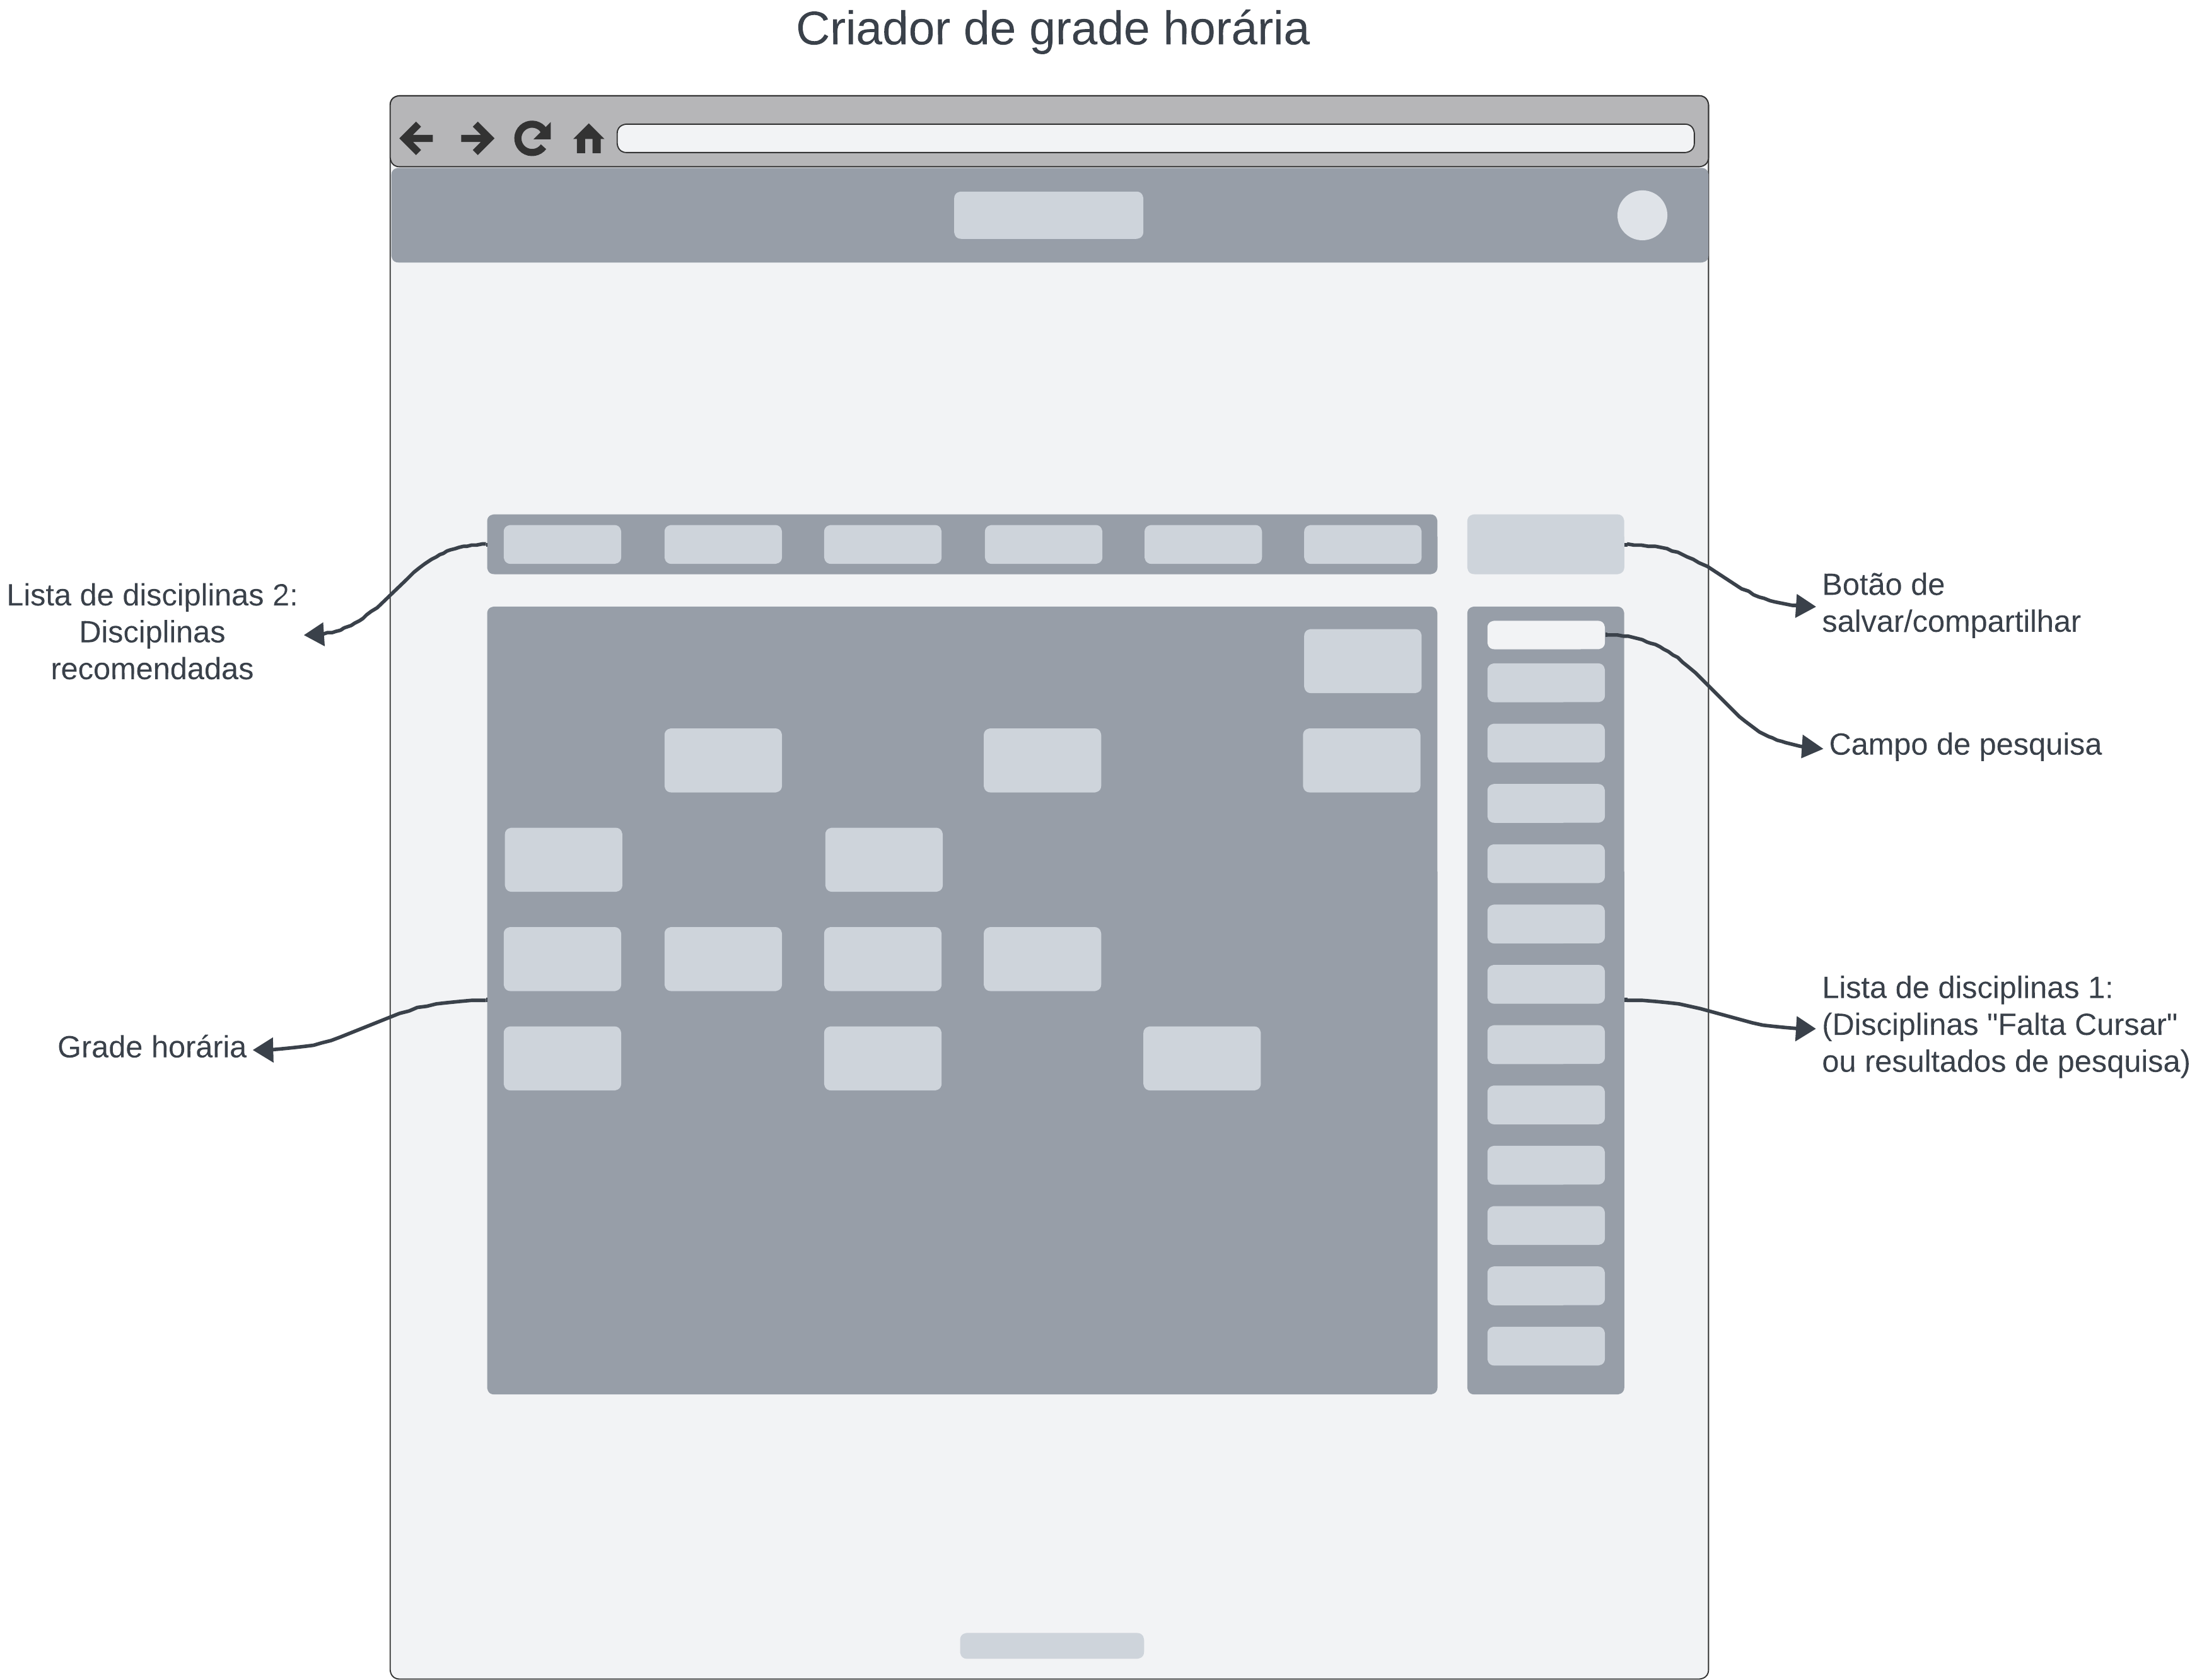
\includegraphics[width=390pt]{figuras/pagina-criacao.png}
    \caption{Wireframe da página de criação de grade horária}
    \label{fig:wireframe-pagina-criacao}
    \end{center}
\end{figure}

\begin{figure}[ht]
    \begin{center}
    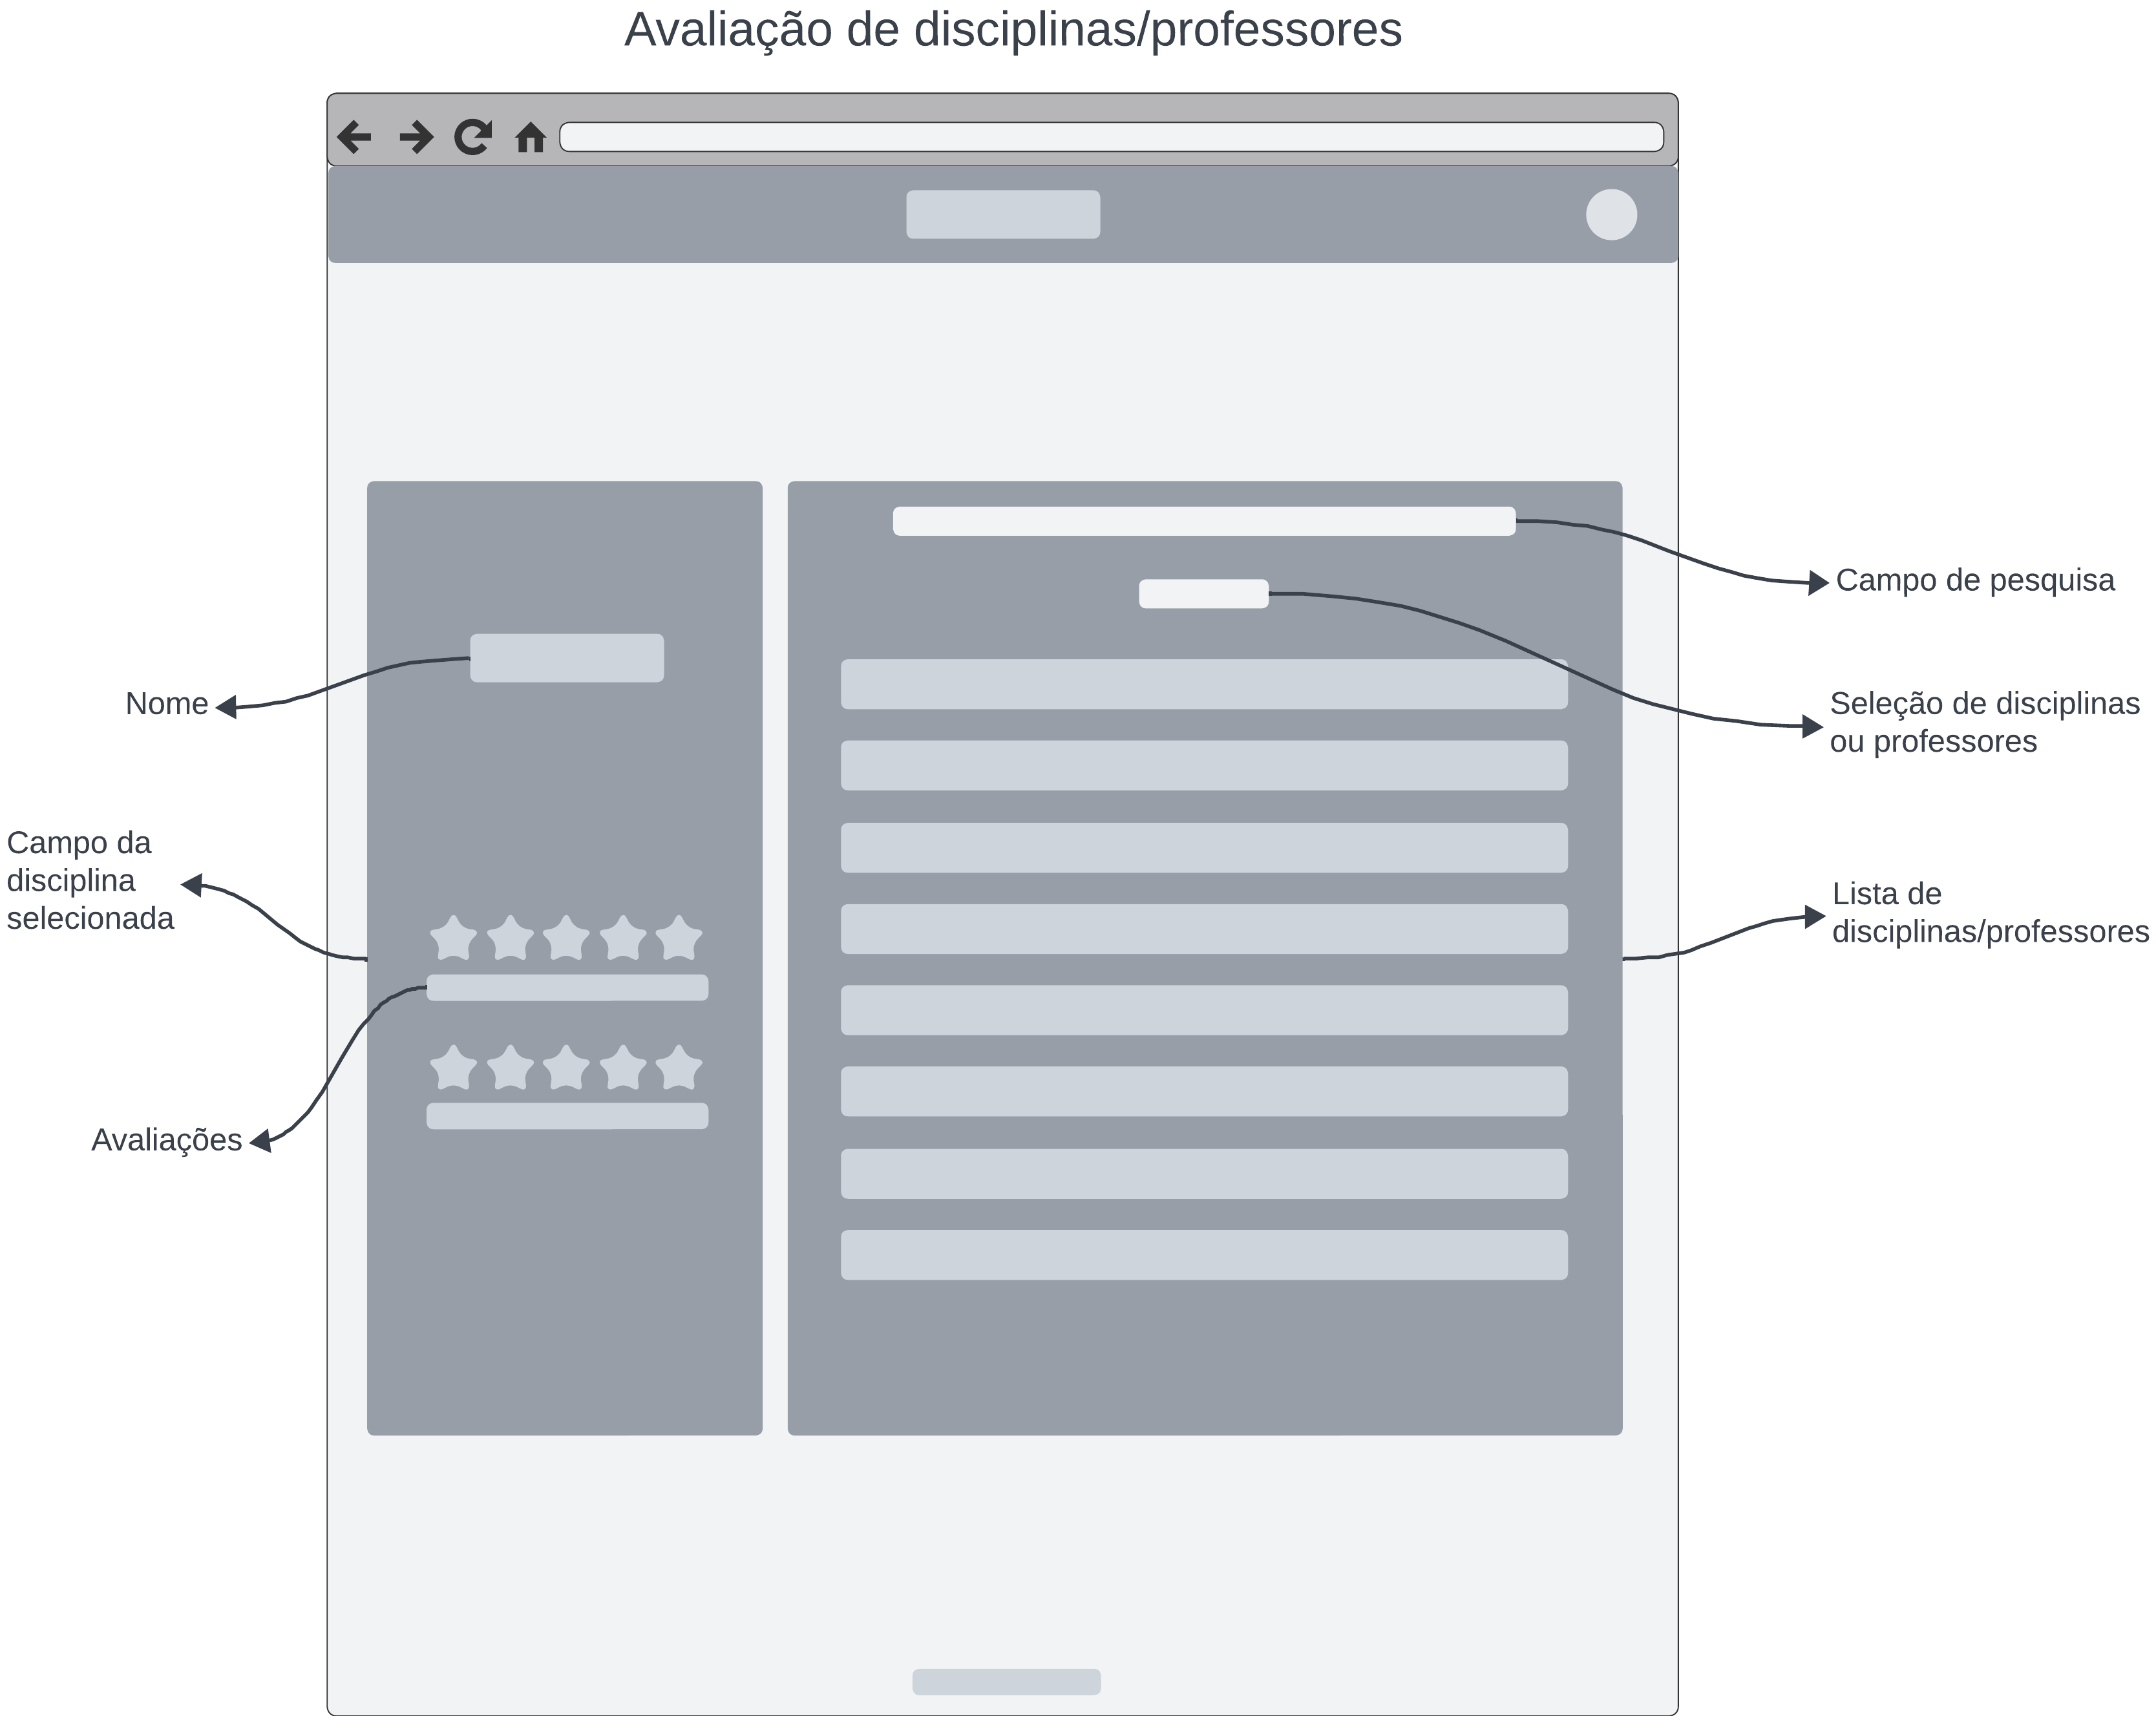
\includegraphics[width=390pt]{figuras/pagina-avaliacao.png}
    \caption{Wireframe da página de avaliação de disciplinas/professores}
    \label{fig:wireframe-pagina-avaliacao}
    \end{center}
\end{figure}